% Options for packages loaded elsewhere
\PassOptionsToPackage{unicode}{hyperref}
\PassOptionsToPackage{hyphens}{url}
\PassOptionsToPackage{dvipsnames,svgnames,x11names}{xcolor}
%
\documentclass[
  10pt,
  ignorenonframetext,
  aspectratio=169]{beamer}
\usepackage{pgfpages}
\setbeamertemplate{caption}[numbered]
\setbeamertemplate{caption label separator}{: }
\setbeamercolor{caption name}{fg=normal text.fg}
\beamertemplatenavigationsymbolsempty
% Prevent slide breaks in the middle of a paragraph
\widowpenalties 1 10000
\raggedbottom
\setbeamertemplate{part page}{
  \centering
  \begin{beamercolorbox}[sep=16pt,center]{part title}
    \usebeamerfont{part title}\insertpart\par
  \end{beamercolorbox}
}
\setbeamertemplate{section page}{
  \centering
  \begin{beamercolorbox}[sep=12pt,center]{part title}
    \usebeamerfont{section title}\insertsection\par
  \end{beamercolorbox}
}
\setbeamertemplate{subsection page}{
  \centering
  \begin{beamercolorbox}[sep=8pt,center]{part title}
    \usebeamerfont{subsection title}\insertsubsection\par
  \end{beamercolorbox}
}
\AtBeginPart{
  \frame{\partpage}
}
\AtBeginSection{
  \ifbibliography
  \else
    \frame{\sectionpage}
  \fi
}
\AtBeginSubsection{
  \frame{\subsectionpage}
}
\usepackage{amsmath,amssymb}
\usepackage{lmodern}
\usepackage{iftex}
\ifPDFTeX
  \usepackage[T1]{fontenc}
  \usepackage[utf8]{inputenc}
  \usepackage{textcomp} % provide euro and other symbols
\else % if luatex or xetex
  \usepackage{unicode-math}
  \defaultfontfeatures{Scale=MatchLowercase}
  \defaultfontfeatures[\rmfamily]{Ligatures=TeX,Scale=1}
\fi
\usetheme[]{Singapore}
% Use upquote if available, for straight quotes in verbatim environments
\IfFileExists{upquote.sty}{\usepackage{upquote}}{}
\IfFileExists{microtype.sty}{% use microtype if available
  \usepackage[]{microtype}
  \UseMicrotypeSet[protrusion]{basicmath} % disable protrusion for tt fonts
}{}
\makeatletter
\@ifundefined{KOMAClassName}{% if non-KOMA class
  \IfFileExists{parskip.sty}{%
    \usepackage{parskip}
  }{% else
    \setlength{\parindent}{0pt}
    \setlength{\parskip}{6pt plus 2pt minus 1pt}}
}{% if KOMA class
  \KOMAoptions{parskip=half}}
\makeatother
\usepackage{xcolor}
\newif\ifbibliography
\usepackage{color}
\usepackage{fancyvrb}
\newcommand{\VerbBar}{|}
\newcommand{\VERB}{\Verb[commandchars=\\\{\}]}
\DefineVerbatimEnvironment{Highlighting}{Verbatim}{commandchars=\\\{\}}
% Add ',fontsize=\small' for more characters per line
\usepackage{framed}
\definecolor{shadecolor}{RGB}{48,48,48}
\newenvironment{Shaded}{\begin{snugshade}}{\end{snugshade}}
\newcommand{\AlertTok}[1]{\textcolor[rgb]{1.00,0.81,0.69}{#1}}
\newcommand{\AnnotationTok}[1]{\textcolor[rgb]{0.50,0.62,0.50}{\textbf{#1}}}
\newcommand{\AttributeTok}[1]{\textcolor[rgb]{0.80,0.80,0.80}{#1}}
\newcommand{\BaseNTok}[1]{\textcolor[rgb]{0.86,0.64,0.64}{#1}}
\newcommand{\BuiltInTok}[1]{\textcolor[rgb]{0.80,0.80,0.80}{#1}}
\newcommand{\CharTok}[1]{\textcolor[rgb]{0.86,0.64,0.64}{#1}}
\newcommand{\CommentTok}[1]{\textcolor[rgb]{0.50,0.62,0.50}{#1}}
\newcommand{\CommentVarTok}[1]{\textcolor[rgb]{0.50,0.62,0.50}{\textbf{#1}}}
\newcommand{\ConstantTok}[1]{\textcolor[rgb]{0.86,0.64,0.64}{\textbf{#1}}}
\newcommand{\ControlFlowTok}[1]{\textcolor[rgb]{0.94,0.87,0.69}{#1}}
\newcommand{\DataTypeTok}[1]{\textcolor[rgb]{0.87,0.87,0.75}{#1}}
\newcommand{\DecValTok}[1]{\textcolor[rgb]{0.86,0.86,0.80}{#1}}
\newcommand{\DocumentationTok}[1]{\textcolor[rgb]{0.50,0.62,0.50}{#1}}
\newcommand{\ErrorTok}[1]{\textcolor[rgb]{0.76,0.75,0.62}{#1}}
\newcommand{\ExtensionTok}[1]{\textcolor[rgb]{0.80,0.80,0.80}{#1}}
\newcommand{\FloatTok}[1]{\textcolor[rgb]{0.75,0.75,0.82}{#1}}
\newcommand{\FunctionTok}[1]{\textcolor[rgb]{0.94,0.94,0.56}{#1}}
\newcommand{\ImportTok}[1]{\textcolor[rgb]{0.80,0.80,0.80}{#1}}
\newcommand{\InformationTok}[1]{\textcolor[rgb]{0.50,0.62,0.50}{\textbf{#1}}}
\newcommand{\KeywordTok}[1]{\textcolor[rgb]{0.94,0.87,0.69}{#1}}
\newcommand{\NormalTok}[1]{\textcolor[rgb]{0.80,0.80,0.80}{#1}}
\newcommand{\OperatorTok}[1]{\textcolor[rgb]{0.94,0.94,0.82}{#1}}
\newcommand{\OtherTok}[1]{\textcolor[rgb]{0.94,0.94,0.56}{#1}}
\newcommand{\PreprocessorTok}[1]{\textcolor[rgb]{1.00,0.81,0.69}{\textbf{#1}}}
\newcommand{\RegionMarkerTok}[1]{\textcolor[rgb]{0.80,0.80,0.80}{#1}}
\newcommand{\SpecialCharTok}[1]{\textcolor[rgb]{0.86,0.64,0.64}{#1}}
\newcommand{\SpecialStringTok}[1]{\textcolor[rgb]{0.80,0.58,0.58}{#1}}
\newcommand{\StringTok}[1]{\textcolor[rgb]{0.80,0.58,0.58}{#1}}
\newcommand{\VariableTok}[1]{\textcolor[rgb]{0.80,0.80,0.80}{#1}}
\newcommand{\VerbatimStringTok}[1]{\textcolor[rgb]{0.80,0.58,0.58}{#1}}
\newcommand{\WarningTok}[1]{\textcolor[rgb]{0.50,0.62,0.50}{\textbf{#1}}}
\usepackage{graphicx}
\makeatletter
\def\maxwidth{\ifdim\Gin@nat@width>\linewidth\linewidth\else\Gin@nat@width\fi}
\def\maxheight{\ifdim\Gin@nat@height>\textheight\textheight\else\Gin@nat@height\fi}
\makeatother
% Scale images if necessary, so that they will not overflow the page
% margins by default, and it is still possible to overwrite the defaults
% using explicit options in \includegraphics[width, height, ...]{}
\setkeys{Gin}{width=\maxwidth,height=\maxheight,keepaspectratio}
% Set default figure placement to htbp
\makeatletter
\def\fps@figure{htbp}
\makeatother
\setlength{\emergencystretch}{3em} % prevent overfull lines
\providecommand{\tightlist}{%
  \setlength{\itemsep}{0pt}\setlength{\parskip}{0pt}}
\setcounter{secnumdepth}{-\maxdimen} % remove section numbering
\newenvironment{cols}[1][]{}{}

\newenvironment{col}[1]{\begin{minipage}{#1}\ignorespaces}{%
\end{minipage}
\ifhmode\unskip\fi
\aftergroup\useignorespacesandallpars}

\def\useignorespacesandallpars#1\ignorespaces\fi{%
#1\fi\ignorespacesandallpars}

\makeatletter
\def\ignorespacesandallpars{%
  \@ifnextchar\par
    {\expandafter\ignorespacesandallpars\@gobble}%
    {}%
}
\makeatother
\ifLuaTeX
  \usepackage{selnolig}  % disable illegal ligatures
\fi
\usepackage[]{natbib}
\bibliographystyle{plainnat}
\IfFileExists{bookmark.sty}{\usepackage{bookmark}}{\usepackage{hyperref}}
\IfFileExists{xurl.sty}{\usepackage{xurl}}{} % add URL line breaks if available
\urlstyle{same} % disable monospaced font for URLs
\hypersetup{
  pdftitle={Text similarity and dimensionality reduction},
  pdfauthor={Max Callaghan},
  colorlinks=true,
  linkcolor={Maroon},
  filecolor={Maroon},
  citecolor={Blue},
  urlcolor={blue},
  pdfcreator={LaTeX via pandoc}}

\title{Text similarity and dimensionality reduction}
\author{Max Callaghan}
\date{2022-10-13}

\begin{document}
\frame{\titlepage}

\hypertarget{introduction-and-objectives}{%
\section{Introduction and
Objectives}\label{introduction-and-objectives}}

\begin{frame}{Intro}
\protect\hypertarget{intro}{}
\begin{cols}

\begin{col}{0.48\textwidth}

\begin{itemize}
  \item<1->The data manipulation tasks were **tricky**.
  \item<2->Don't be afraid to submit imperfect implementations that get us part of the way there
  \item<3->You will likely need loops: remember that the easiest way to get a loop working is to try it out on a single element of the sort you will be looping through.
  \item<4->Getting unstructured texts into data formats is a really important skill for real world text as data work. BUT, our focus shifts now on to what to do with this data.
  \item<5->However, this means we need a bit of maths today
\end{itemize}

\end{col}

\begin{col}{0.04\textwidth}
~

\end{col}

\begin{col}{0.48\textwidth}

\only<5->{

\includegraphics[width=\linewidth]{images/horse.png}
}

\end{col}

\end{cols}
\end{frame}

\begin{frame}{Objectives}
\protect\hypertarget{objectives}{}
By now we have figured out how to \textbf{represent} texts in a
multidimensional space.

In this session we will find out

\begin{itemize}
\tightlist
\item
  how to measure \textbf{similarity} in this space
\item
  how to \textbf{reduce} the \textbf{dimensionality} of this space to
  make it easier to explore and visualise.
\end{itemize}
\end{frame}

\hypertarget{text-similarity-distance}{%
\section{Text similarity \& distance}\label{text-similarity-distance}}

\begin{frame}{Why similarity}
\protect\hypertarget{why-similarity}{}
Why do we want to measure whether texts are similar or different?

\begin{itemize}
  \item<2-> Retrieving relevant but inexact information
  \item<3-> Learning topics or clusters which group similar documents together
  \item<4-> Building a classifier that allocates labels to texts that a similar to our labelled data
\end{itemize}

What does similarity mean?
\end{frame}

\begin{frame}{Properties of a similarity metric}
\protect\hypertarget{properties-of-a-similarity-metric}{}
According to Grimmer, Roberts and Stewart,

\begin{enumerate}
  \item<1-> Maximum similarity should occur when comparing a document to itself
  \item<2-> Two documents that share no words in common should have minimum similarity
  \item<3-> Similarity should increase as more of the same words are used
  \item<4-> The measure should work symmetrically: A is similar to B as B is to A
\end{enumerate}
\end{frame}

\begin{frame}[fragile]{Metrics: Vector representations of texts}
\protect\hypertarget{metrics-vector-representations-of-texts}{}
Let us imagine we have 2 documents, which we represent in a document
feature matrix. If we want to get the \textbf{vector} representation of
each of these documents, we simply take the relevant row

\begin{cols}

\begin{col}{0.48\textwidth}

\scriptsize

\begin{Shaded}
\begin{Highlighting}[]
\FunctionTok{library}\NormalTok{(quanteda)}
\NormalTok{texts }\OtherTok{\textless{}{-}} \FunctionTok{c}\NormalTok{(}\StringTok{"apple orange pear"}\NormalTok{, }\StringTok{"apple pear quince"}\NormalTok{)}
\NormalTok{dfmat }\OtherTok{\textless{}{-}}\NormalTok{ texts }\SpecialCharTok{\%\textgreater{}\%}
  \FunctionTok{tokens}\NormalTok{() }\SpecialCharTok{\%\textgreater{}\%}
  \FunctionTok{dfm}\NormalTok{() }\SpecialCharTok{\%\textgreater{}\%}
  \FunctionTok{as.matrix}\NormalTok{()}
\FunctionTok{print}\NormalTok{(dfmat)}
\end{Highlighting}
\end{Shaded}

\begin{verbatim}
##        features
## docs    apple orange pear quince
##   text1     1      1    1      0
##   text2     1      0    1      1
\end{verbatim}

\begin{Shaded}
\begin{Highlighting}[]
\NormalTok{a }\OtherTok{\textless{}{-}}\NormalTok{ dfmat[}\DecValTok{1}\NormalTok{,]}
\NormalTok{b }\OtherTok{\textless{}{-}}\NormalTok{ dfmat[}\DecValTok{2}\NormalTok{,]}
\FunctionTok{print}\NormalTok{(a)}
\end{Highlighting}
\end{Shaded}

\begin{verbatim}
##  apple orange   pear quince 
##      1      1      1      0
\end{verbatim}

\begin{Shaded}
\begin{Highlighting}[]
\FunctionTok{print}\NormalTok{(b)}
\end{Highlighting}
\end{Shaded}

\begin{verbatim}
##  apple orange   pear quince 
##      1      0      1      1
\end{verbatim}

\end{col}

\begin{col}{0.04\textwidth}
~

\end{col}

\begin{col}{0.48\textwidth}

\scriptsize

\begin{Shaded}
\begin{Highlighting}[]
\ImportTok{from}\NormalTok{ sklearn.feature\_extraction.text }\ImportTok{import}\NormalTok{ CountVectorizer}

\NormalTok{texts }\OperatorTok{=}\NormalTok{ [}\StringTok{"apple orange pear"}\NormalTok{, }\StringTok{"apple pear quince"}\NormalTok{]}
\NormalTok{vec }\OperatorTok{=}\NormalTok{ CountVectorizer()}
\NormalTok{dfmat }\OperatorTok{=}\NormalTok{ vec.fit\_transform(texts).todense()}

\BuiltInTok{print}\NormalTok{(vec.get\_feature\_names\_out())}
\end{Highlighting}
\end{Shaded}

\begin{verbatim}
## ['apple' 'orange' 'pear' 'quince']
\end{verbatim}

\begin{Shaded}
\begin{Highlighting}[]
\BuiltInTok{print}\NormalTok{(dfmat)}
\end{Highlighting}
\end{Shaded}

\begin{verbatim}
## [[1 1 1 0]
##  [1 0 1 1]]
\end{verbatim}

\begin{Shaded}
\begin{Highlighting}[]
\NormalTok{a }\OperatorTok{=}\NormalTok{ dfmat[}\DecValTok{0}\NormalTok{,].A1}
\NormalTok{b }\OperatorTok{=}\NormalTok{ dfmat[}\DecValTok{1}\NormalTok{,].A1}
\BuiltInTok{print}\NormalTok{(a)}
\end{Highlighting}
\end{Shaded}

\begin{verbatim}
## [1 1 1 0]
\end{verbatim}

\begin{Shaded}
\begin{Highlighting}[]
\BuiltInTok{print}\NormalTok{(b)}
\end{Highlighting}
\end{Shaded}

\begin{verbatim}
## [1 0 1 1]
\end{verbatim}

\end{col}

\end{cols}
\end{frame}

\begin{frame}[fragile]{Metrics: The inner product of two vectors}
\protect\hypertarget{metrics-the-inner-product-of-two-vectors}{}
The simplest way to calculate the similarity of two matrices is to
calculate their \textbf{inner product} or \textbf{dot product}, which
means multiply the first element of \(a\) with the first element of
\(b\), and then the second, etc. and then add all these up.

\[\mathbf{a} \cdot \mathbf{b} =a_1b_1 + a_2b_2 + ...\]

\scriptsize

\begin{Shaded}
\begin{Highlighting}[]
\FunctionTok{print}\NormalTok{(a}\SpecialCharTok{*}\NormalTok{b)}
\end{Highlighting}
\end{Shaded}

\begin{verbatim}
##  apple orange   pear quince 
##      1      0      1      0
\end{verbatim}

\begin{Shaded}
\begin{Highlighting}[]
\NormalTok{inner\_product }\OtherTok{=} \FunctionTok{sum}\NormalTok{(a}\SpecialCharTok{*}\NormalTok{b)}
\NormalTok{inner\_product}
\end{Highlighting}
\end{Shaded}

\begin{verbatim}
## [1] 2
\end{verbatim}
\end{frame}

\begin{frame}[fragile]{Metrics: the effect of long texts}
\protect\hypertarget{metrics-the-effect-of-long-texts}{}
Let's imagine we have a much longer text. As long as it has just one
more word in commmon, by this measure it will be more similar.

\scriptsize

\begin{Shaded}
\begin{Highlighting}[]
\NormalTok{texts }\OtherTok{\textless{}{-}} \FunctionTok{c}\NormalTok{(}
  \StringTok{"apple orange pear"}\NormalTok{, }\StringTok{"apple pear quince"}\NormalTok{,}
  \StringTok{"apple pear orange quince peach avocado kiwi physalis"}
\NormalTok{)}
\NormalTok{dfmat }\OtherTok{\textless{}{-}}\NormalTok{ texts }\SpecialCharTok{\%\textgreater{}\%} \FunctionTok{tokens}\NormalTok{() }\SpecialCharTok{\%\textgreater{}\%} \FunctionTok{dfm}\NormalTok{() }\SpecialCharTok{\%\textgreater{}\%} \FunctionTok{as.matrix}\NormalTok{()}
\FunctionTok{print}\NormalTok{(dfmat)}
\end{Highlighting}
\end{Shaded}

\begin{verbatim}
##        features
## docs    apple orange pear quince peach avocado kiwi physalis
##   text1     1      1    1      0     0       0    0        0
##   text2     1      0    1      1     0       0    0        0
##   text3     1      1    1      1     1       1    1        1
\end{verbatim}

\begin{Shaded}
\begin{Highlighting}[]
\NormalTok{a }\OtherTok{\textless{}{-}}\NormalTok{ dfmat[}\DecValTok{1}\NormalTok{,]}
\NormalTok{b }\OtherTok{\textless{}{-}}\NormalTok{ dfmat[}\DecValTok{2}\NormalTok{,]}
\NormalTok{c }\OtherTok{\textless{}{-}}\NormalTok{ dfmat[}\DecValTok{3}\NormalTok{,]}
\FunctionTok{print}\NormalTok{(a}\SpecialCharTok{*}\NormalTok{c)}
\end{Highlighting}
\end{Shaded}

\begin{verbatim}
##    apple   orange     pear   quince    peach  avocado     kiwi physalis 
##        1        1        1        0        0        0        0        0
\end{verbatim}

\begin{Shaded}
\begin{Highlighting}[]
\FunctionTok{print}\NormalTok{(}\FunctionTok{sum}\NormalTok{(a}\SpecialCharTok{*}\NormalTok{c))}
\end{Highlighting}
\end{Shaded}

\begin{verbatim}
## [1] 3
\end{verbatim}
\end{frame}

\begin{frame}[fragile]{Metrics: controlling for magnitude}
\protect\hypertarget{metrics-controlling-for-magnitude}{}
We can compute the magnitude of a vector (denoted \(||\mathbf{a}||\)),
by taking the square root of the inner product with itself

\[||\mathbf{a}|| = \sqrt{\mathbf{a} \cdot \mathbf{a}} \]

\scriptsize

\begin{Shaded}
\begin{Highlighting}[]
\FunctionTok{print}\NormalTok{(a}\SpecialCharTok{*}\NormalTok{a)}
\end{Highlighting}
\end{Shaded}

\begin{verbatim}
##    apple   orange     pear   quince    peach  avocado     kiwi physalis 
##        1        1        1        0        0        0        0        0
\end{verbatim}

\begin{Shaded}
\begin{Highlighting}[]
\FunctionTok{print}\NormalTok{(}\FunctionTok{sqrt}\NormalTok{(}\FunctionTok{sum}\NormalTok{(a}\SpecialCharTok{*}\NormalTok{a)))}
\end{Highlighting}
\end{Shaded}

\begin{verbatim}
## [1] 1.732051
\end{verbatim}

\begin{Shaded}
\begin{Highlighting}[]
\FunctionTok{print}\NormalTok{(c}\SpecialCharTok{*}\NormalTok{c)}
\end{Highlighting}
\end{Shaded}

\begin{verbatim}
##    apple   orange     pear   quince    peach  avocado     kiwi physalis 
##        1        1        1        1        1        1        1        1
\end{verbatim}

\begin{Shaded}
\begin{Highlighting}[]
\FunctionTok{print}\NormalTok{(}\FunctionTok{sqrt}\NormalTok{(}\FunctionTok{sum}\NormalTok{(c}\SpecialCharTok{*}\NormalTok{c)))}
\end{Highlighting}
\end{Shaded}

\begin{verbatim}
## [1] 2.828427
\end{verbatim}
\end{frame}

\begin{frame}[fragile]{Metrics: cosine similarity}
\protect\hypertarget{metrics-cosine-similarity}{}
We can calculate what we call the \textbf{cosine similarity} by taking
the \textbf{inner product} of two \textbf{magnitude normalized} vectors.

\begin{cols}

\begin{col}{0.315\textwidth}
\[ cos(\theta) = \frac{\mathbf{a}}{||\mathbf{a}||} \cdot \frac{\mathbf{b}}{||\mathbf{b}||}\]

\end{col}

\begin{col}{0.05\textwidth}
~

\end{col}

\begin{col}{0.68\textwidth}

\scriptsize

\begin{Shaded}
\begin{Highlighting}[]
\NormalTok{norm\_a }\OtherTok{\textless{}{-}}\NormalTok{ a}\SpecialCharTok{/}\FunctionTok{sqrt}\NormalTok{(}\FunctionTok{sum}\NormalTok{(a}\SpecialCharTok{*}\NormalTok{a))}
\FunctionTok{print}\NormalTok{(norm\_a)}
\end{Highlighting}
\end{Shaded}

\begin{verbatim}
##     apple    orange      pear    quince     peach   avocado      kiwi  physalis 
## 0.5773503 0.5773503 0.5773503 0.0000000 0.0000000 0.0000000 0.0000000 0.0000000
\end{verbatim}

\begin{Shaded}
\begin{Highlighting}[]
\NormalTok{norm\_b }\OtherTok{\textless{}{-}}\NormalTok{ b}\SpecialCharTok{/}\FunctionTok{sqrt}\NormalTok{(}\FunctionTok{sum}\NormalTok{(b}\SpecialCharTok{*}\NormalTok{b))}
\FunctionTok{print}\NormalTok{(norm\_b)}
\end{Highlighting}
\end{Shaded}

\begin{verbatim}
##     apple    orange      pear    quince     peach   avocado      kiwi  physalis 
## 0.5773503 0.0000000 0.5773503 0.5773503 0.0000000 0.0000000 0.0000000 0.0000000
\end{verbatim}

\begin{Shaded}
\begin{Highlighting}[]
\NormalTok{norm\_c }\OtherTok{\textless{}{-}}\NormalTok{ c}\SpecialCharTok{/}\FunctionTok{sqrt}\NormalTok{(}\FunctionTok{sum}\NormalTok{(c}\SpecialCharTok{*}\NormalTok{c))}
\FunctionTok{print}\NormalTok{(norm\_c)}
\end{Highlighting}
\end{Shaded}

\begin{verbatim}
##     apple    orange      pear    quince     peach   avocado      kiwi  physalis 
## 0.3535534 0.3535534 0.3535534 0.3535534 0.3535534 0.3535534 0.3535534 0.3535534
\end{verbatim}

\begin{Shaded}
\begin{Highlighting}[]
\FunctionTok{print}\NormalTok{(}\FunctionTok{sum}\NormalTok{(norm\_a}\SpecialCharTok{*}\NormalTok{norm\_b))}
\end{Highlighting}
\end{Shaded}

\begin{verbatim}
## [1] 0.6666667
\end{verbatim}

\begin{Shaded}
\begin{Highlighting}[]
\FunctionTok{print}\NormalTok{(}\FunctionTok{sum}\NormalTok{(norm\_a}\SpecialCharTok{*}\NormalTok{norm\_c))}
\end{Highlighting}
\end{Shaded}

\begin{verbatim}
## [1] 0.6123724
\end{verbatim}

\end{col}

\end{cols}
\end{frame}

\begin{frame}[fragile]{Metrics: cosine similarity II}
\protect\hypertarget{metrics-cosine-similarity-ii}{}
Let's create a document feature matrix with only 2 dimensions

\begin{Shaded}
\begin{Highlighting}[]
\ImportTok{from}\NormalTok{ sklearn.feature\_extraction.text }\ImportTok{import}\NormalTok{ CountVectorizer}
\NormalTok{texts }\OperatorTok{=}\NormalTok{ [}\StringTok{"apple pear"}\NormalTok{,}\StringTok{"apple pear apple pear"}\NormalTok{,}\StringTok{"apple apple"}\NormalTok{]}
\NormalTok{textnames }\OperatorTok{=}\NormalTok{ [}\StringTok{"A"}\NormalTok{,}\StringTok{"B"}\NormalTok{,}\StringTok{"C"}\NormalTok{]}
\NormalTok{vec }\OperatorTok{=}\NormalTok{ CountVectorizer()}
\NormalTok{dfmat }\OperatorTok{=}\NormalTok{ vec.fit\_transform(texts).todense()}
\NormalTok{a }\OperatorTok{=}\NormalTok{ dfmat[}\DecValTok{0}\NormalTok{,].A1}
\NormalTok{b }\OperatorTok{=}\NormalTok{ dfmat[}\DecValTok{1}\NormalTok{,].A1}
\NormalTok{c }\OperatorTok{=}\NormalTok{ dfmat[}\DecValTok{2}\NormalTok{,].A1}
\NormalTok{dfmat}
\end{Highlighting}
\end{Shaded}

\begin{verbatim}
## matrix([[1, 1],
##         [2, 2],
##         [2, 0]])
\end{verbatim}
\end{frame}

\begin{frame}[fragile]{Metrics: cosine similarity III}
\protect\hypertarget{metrics-cosine-similarity-iii}{}
\begin{cols}

\begin{col}{0.68\textwidth}

\medskip

\scriptsize

\begin{Shaded}
\begin{Highlighting}[]
\ImportTok{import}\NormalTok{ matplotlib.pyplot }\ImportTok{as}\NormalTok{ plt}
\NormalTok{fig, ax }\OperatorTok{=}\NormalTok{ plt.subplots(figsize}\OperatorTok{=}\NormalTok{(}\FloatTok{3.5}\NormalTok{,}\FloatTok{3.5}\NormalTok{))}
\ControlFlowTok{for}\NormalTok{ i, row }\KeywordTok{in} \BuiltInTok{enumerate}\NormalTok{(dfmat):}
\NormalTok{    x }\OperatorTok{=}\NormalTok{ row.A1[}\DecValTok{0}\NormalTok{]}
\NormalTok{    y }\OperatorTok{=}\NormalTok{ row.A1[}\DecValTok{1}\NormalTok{]}
\NormalTok{    ax.arrow(}\DecValTok{0}\NormalTok{,}\DecValTok{0}\NormalTok{,x,y,head\_width}\OperatorTok{=}\FloatTok{0.08}\NormalTok{)}
\NormalTok{    ax.text(x}\OperatorTok{{-}}\FloatTok{0.1}\NormalTok{,y}\OperatorTok{+}\FloatTok{0.05}\NormalTok{,textnames[i])}
\NormalTok{ax.set\_aspect(}\StringTok{"equal"}\NormalTok{)}
\NormalTok{plt.savefig(}\StringTok{"plots/cosine\_similarity.png"}\NormalTok{)}
\end{Highlighting}
\end{Shaded}

\end{col}

\begin{col}{0.04\textwidth}
~

\end{col}

\begin{col}{0.28\textwidth}
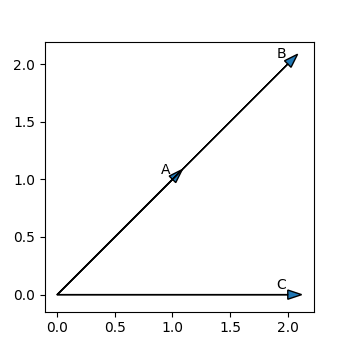
\includegraphics{plots/cosine_similarity.png}

\end{col}

\end{cols}

\scriptsize

\begin{Shaded}
\begin{Highlighting}[]
\ImportTok{import}\NormalTok{ numpy }\ImportTok{as}\NormalTok{ np}
\NormalTok{cosine\_sim }\OperatorTok{=}\NormalTok{ np.cos(np.radians(}\DecValTok{45}\NormalTok{))}
\BuiltInTok{print}\NormalTok{(cosine\_sim)}
\end{Highlighting}
\end{Shaded}

\begin{verbatim}
## 0.7071067811865476
\end{verbatim}

\begin{Shaded}
\begin{Highlighting}[]
\KeywordTok{def}\NormalTok{ normed\_inner\_prod(a,b):}
\NormalTok{  norm\_a }\OperatorTok{=}\NormalTok{ np.sqrt(}\BuiltInTok{sum}\NormalTok{(a}\OperatorTok{*}\NormalTok{a))}
\NormalTok{  norm\_b }\OperatorTok{=}\NormalTok{ np.sqrt(}\BuiltInTok{sum}\NormalTok{(b}\OperatorTok{*}\NormalTok{b))}
  \ControlFlowTok{return} \BuiltInTok{sum}\NormalTok{(a}\OperatorTok{/}\NormalTok{norm\_a }\OperatorTok{*}\NormalTok{ b}\OperatorTok{/}\NormalTok{norm\_b)}
\NormalTok{normed\_inner\_prod(a,c)}
\end{Highlighting}
\end{Shaded}

\begin{verbatim}
## 0.7071067811865475
\end{verbatim}
\end{frame}

\begin{frame}[fragile]{Metrics: cosine similarity IV}
\protect\hypertarget{metrics-cosine-similarity-iv}{}
\begin{cols}

\begin{col}{0.63\textwidth}

\medskip

\scriptsize

\begin{Shaded}
\begin{Highlighting}[]
\ImportTok{from}\NormalTok{ matplotlib.colors }\ImportTok{import}\NormalTok{ CenteredNorm}
\ImportTok{import}\NormalTok{ matplotlib.cm }\ImportTok{as}\NormalTok{ cm}
\NormalTok{colormap }\OperatorTok{=}\NormalTok{ cm.RdBu}
\NormalTok{norm }\OperatorTok{=}\NormalTok{ CenteredNorm()}

\NormalTok{fig, ax }\OperatorTok{=}\NormalTok{ plt.subplots(figsize}\OperatorTok{=}\NormalTok{(}\DecValTok{4}\NormalTok{,}\DecValTok{4}\NormalTok{))}

\NormalTok{degrees }\OperatorTok{=} \BuiltInTok{range}\NormalTok{(}\DecValTok{360}\NormalTok{)}
\NormalTok{radians }\OperatorTok{=}\NormalTok{ np.radians(degrees)}
\NormalTok{x }\OperatorTok{=} \DecValTok{1}\OperatorTok{*}\NormalTok{np.cos(radians)}
\NormalTok{y }\OperatorTok{=} \DecValTok{1}\OperatorTok{*}\NormalTok{np.sin(radians)}
\NormalTok{similarity }\OperatorTok{=}\NormalTok{ np.cos(radians)}
   
\NormalTok{circ }\OperatorTok{=}\NormalTok{ ax.scatter(x,y, c}\OperatorTok{=}\NormalTok{similarity, norm}\OperatorTok{=}\NormalTok{norm, cmap}\OperatorTok{=}\NormalTok{colormap)}
    
\NormalTok{ax.set\_aspect(}\StringTok{"equal"}\NormalTok{)}
\NormalTok{plt.colorbar(circ)}
\end{Highlighting}
\end{Shaded}

\begin{Shaded}
\begin{Highlighting}[]
\NormalTok{plt.savefig(}\StringTok{"plots/cosine\_similarity\_distribution.png"}\NormalTok{, bbox\_inches}\OperatorTok{=}\StringTok{"tight"}\NormalTok{)}
\end{Highlighting}
\end{Shaded}

\end{col}

\begin{col}{0.04\textwidth}
~

\end{col}

\begin{col}{0.33\textwidth}
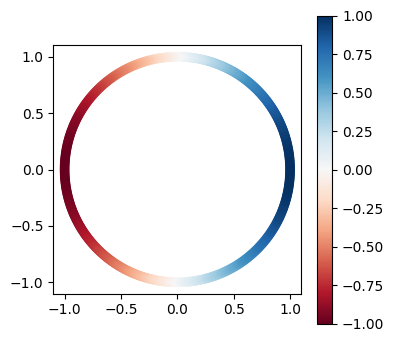
\includegraphics{plots/cosine_similarity_distribution.png}

\end{col}

\end{cols}
\end{frame}

\begin{frame}{Exercise}
\protect\hypertarget{exercise}{}
Let's try to build a chain of texts that starts at

``Central bankers signal intention to press ahead with aggressive
campaign to tighten monetary policy''

and ends at

``SpaceX's Starlink terminals in Ukraine back online after outages''

We want to ensure each text in the chain has a similarity to the
previous text that fulfils the condition

\[0.5 < cos(\theta) < 1\]
\end{frame}

\begin{frame}{Euclidean distance}
\protect\hypertarget{euclidean-distance}{}
The Euclidean distance between two points is the length of a line
segment between those points.

\begin{cols}

\begin{col}{0.63\textwidth}

How would we calculate the length of the line between A and B?

\only<2->{Pythagoras!}

\end{col}

\begin{col}{0.04\textwidth}
~

\end{col}

\begin{col}{0.33\textwidth}
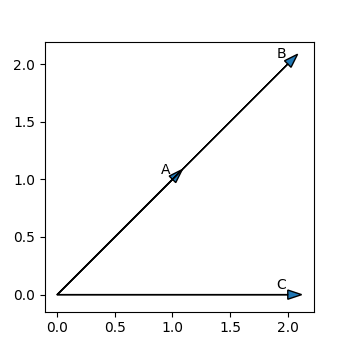
\includegraphics{plots/cosine_similarity.png}

\end{col}

\end{cols}
\end{frame}

\begin{frame}[fragile]{Euclidean distance}
\protect\hypertarget{euclidean-distance-1}{}
The Euclidean distance between two points is the length of a line
segment between those points.

\begin{cols}

\begin{col}{0.63\textwidth}

How would we calculate the line between A and B?

\[d(p,q) = \sqrt{(q_1-p_1)^2 + (q_2-p_2)^2}\]

\begin{Shaded}
\begin{Highlighting}[]
\NormalTok{np.sqrt((a[}\DecValTok{0}\NormalTok{]}\OperatorTok{{-}}\NormalTok{b[}\DecValTok{0}\NormalTok{])}\OperatorTok{**}\DecValTok{2} \OperatorTok{+}\NormalTok{ (a[}\DecValTok{1}\NormalTok{]}\OperatorTok{{-}}\NormalTok{b[}\DecValTok{1}\NormalTok{])}\OperatorTok{**}\DecValTok{2}\NormalTok{)}
\end{Highlighting}
\end{Shaded}

\begin{verbatim}
## 1.4142135623730951
\end{verbatim}

\end{col}

\begin{col}{0.04\textwidth}
~

\end{col}

\begin{col}{0.33\textwidth}
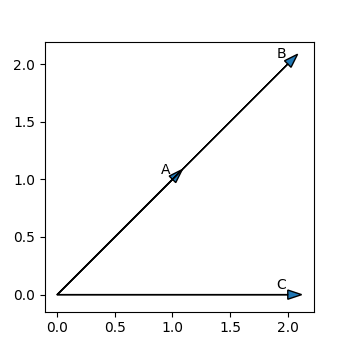
\includegraphics{plots/cosine_similarity.png}

\end{col}

\end{cols}
\end{frame}

\begin{frame}[fragile]{Computing similarity}
\protect\hypertarget{computing-similarity}{}
We can compute similarity or distance using any common metric, and get
the result as a matrix of pairwise comparisons.

\scriptsize

\begin{Shaded}
\begin{Highlighting}[]
\FunctionTok{library}\NormalTok{(quanteda.textstats)}
\NormalTok{texts }\OtherTok{\textless{}{-}} \FunctionTok{c}\NormalTok{(}
  \StringTok{"apple orange pear"}\NormalTok{, }\StringTok{"apple pear quince"}\NormalTok{,}
  \StringTok{"apple pear orange quince peach avocado kiwi physalis"}
\NormalTok{)}
\NormalTok{dfmat }\OtherTok{\textless{}{-}}\NormalTok{ texts }\SpecialCharTok{\%\textgreater{}\%} \FunctionTok{tokens}\NormalTok{() }\SpecialCharTok{\%\textgreater{}\%} \FunctionTok{dfm}\NormalTok{()}
\FunctionTok{textstat\_simil}\NormalTok{(dfmat, }\AttributeTok{method=}\StringTok{"cosine"}\NormalTok{)}
\end{Highlighting}
\end{Shaded}

\begin{verbatim}
## textstat_simil object; method = "cosine"
##       text1 text2 text3
## text1 1.000 0.667 0.612
## text2 0.667 1.000 0.612
## text3 0.612 0.612 1.000
\end{verbatim}
\end{frame}

\begin{frame}[fragile]{Computing similarity}
\protect\hypertarget{computing-similarity-1}{}
We can compute similarity or distance using any common metric, and get
the result as a matrix of pairwise comparisons. Putting this matrix into
as.data.frame gives us all these combinations row by row.

\scriptsize

\begin{Shaded}
\begin{Highlighting}[]
\FunctionTok{library}\NormalTok{(quanteda.textstats)}
\NormalTok{texts }\OtherTok{\textless{}{-}} \FunctionTok{c}\NormalTok{(}
  \StringTok{"apple orange pear"}\NormalTok{, }\StringTok{"apple pear quince"}\NormalTok{,}
  \StringTok{"apple pear orange quince peach avocado kiwi physalis"}
\NormalTok{)}
\NormalTok{dfmat }\OtherTok{\textless{}{-}}\NormalTok{ texts }\SpecialCharTok{\%\textgreater{}\%} \FunctionTok{tokens}\NormalTok{() }\SpecialCharTok{\%\textgreater{}\%} \FunctionTok{dfm}\NormalTok{()}
\NormalTok{sims }\OtherTok{\textless{}{-}} \FunctionTok{textstat\_simil}\NormalTok{(dfmat, }\AttributeTok{method=}\StringTok{"cosine"}\NormalTok{)}
\NormalTok{df }\OtherTok{\textless{}{-}} \FunctionTok{as.data.frame}\NormalTok{(sims, }\AttributeTok{upper=}\ConstantTok{TRUE}\NormalTok{)}
\NormalTok{df}
\end{Highlighting}
\end{Shaded}

\begin{verbatim}
##   document1 document2    cosine
## 1     text2     text1 0.6666667
## 2     text3     text1 0.6123724
## 3     text1     text2 0.6666667
## 4     text3     text2 0.6123724
## 5     text1     text3 0.6123724
## 6     text2     text3 0.6123724
\end{verbatim}
\end{frame}

\begin{frame}[fragile]{Computing similarity in python}
\protect\hypertarget{computing-similarity-in-python}{}
In python we can use the pairwise metrics from scikitlearn.

\scriptsize

\begin{Shaded}
\begin{Highlighting}[]
\ImportTok{from}\NormalTok{ sklearn.metrics.pairwise }\ImportTok{import}\NormalTok{ cosine\_similarity}
\ImportTok{from}\NormalTok{ sklearn.metrics.pairwise }\ImportTok{import}\NormalTok{ euclidean\_distances}
\NormalTok{texts }\OperatorTok{=}\NormalTok{ [}
  \StringTok{"apple orange pear"}\NormalTok{, }\StringTok{"apple pear quince"}\NormalTok{,}
  \StringTok{"apple pear orange quince peach avocado kiwi physalis"}
\NormalTok{]}
\NormalTok{vec }\OperatorTok{=}\NormalTok{ CountVectorizer()}
\NormalTok{dfmat }\OperatorTok{=}\NormalTok{ vec.fit\_transform(texts)}
\NormalTok{dist\_dfmat }\OperatorTok{=}\NormalTok{ cosine\_similarity(dfmat)}
\NormalTok{dist\_dfmat}
\end{Highlighting}
\end{Shaded}

\begin{verbatim}
## array([[1.        , 0.66666667, 0.61237244],
##        [0.66666667, 1.        , 0.61237244],
##        [0.61237244, 0.61237244, 1.        ]])
\end{verbatim}
\end{frame}

\begin{frame}[fragile]{Computing similarity in python}
\protect\hypertarget{computing-similarity-in-python-1}{}
Getting the most similar text to a given text requires setting the
diagonal values to NaN. Then, for a given row, we can apply
\texttt{argsort} to a negated version of the array. This gives us the
indices of the elements in descending order of similarity

\scriptsize

\begin{Shaded}
\begin{Highlighting}[]
\ImportTok{from}\NormalTok{ sklearn.metrics.pairwise }\ImportTok{import}\NormalTok{ cosine\_similarity}
\ImportTok{from}\NormalTok{ sklearn.metrics.pairwise }\ImportTok{import}\NormalTok{ euclidean\_distances}
\NormalTok{texts }\OperatorTok{=}\NormalTok{ [}
  \StringTok{"apple orange pear"}\NormalTok{, }\StringTok{"apple pear quince"}\NormalTok{,}
  \StringTok{"apple pear orange quince peach avocado kiwi physalis"}
\NormalTok{]}
\NormalTok{vec }\OperatorTok{=}\NormalTok{ CountVectorizer()}
\NormalTok{dfmat }\OperatorTok{=}\NormalTok{ vec.fit\_transform(texts)}
\NormalTok{dist\_dfmat }\OperatorTok{=}\NormalTok{ cosine\_similarity(dfmat)}
\NormalTok{np.fill\_diagonal(dist\_dfmat,np.NaN)}
\BuiltInTok{print}\NormalTok{(}\OperatorTok{{-}}\NormalTok{dist\_dfmat)}
\end{Highlighting}
\end{Shaded}

\begin{verbatim}
## [[        nan -0.66666667 -0.61237244]
##  [-0.66666667         nan -0.61237244]
##  [-0.61237244 -0.61237244         nan]]
\end{verbatim}

\begin{Shaded}
\begin{Highlighting}[]
\NormalTok{np.argsort(}\OperatorTok{{-}}\NormalTok{dist\_dfmat[}\DecValTok{0}\NormalTok{])}
\end{Highlighting}
\end{Shaded}

\begin{verbatim}
## array([1, 2, 0])
\end{verbatim}
\end{frame}

\begin{frame}[fragile]{Retrieving the most similar texts}
\protect\hypertarget{retrieving-the-most-similar-texts}{}
I've downloaded the manifestos from 4 UK political parties from the last
election from the WZB manifesto project. You will find them in
\texttt{data/uk\_manifestos.csv}. I'd like you to

\begin{itemize}
\tightlist
\item
  Read in the texts (each text is a sentence from a manifesto)
\item
  Calculate the similarity matrix
\item
  Choose a text you find interesting
\item
  Retrieve the most similar texts to that one
\end{itemize}
\end{frame}

\hypertarget{dimensionality-reduction}{%
\section{Dimensionality reduction}\label{dimensionality-reduction}}

\begin{frame}{Rationale}
\protect\hypertarget{rationale}{}
We represent documents in a multidimensional space but it is abstract
and hard to visualise.

What if there was a way to represent documents in a 2-dimensional space
that preserves some of the relationships between documents in a
multi-dimensional space?

Then we could make nice plots!
\end{frame}

\begin{frame}{}
\protect\hypertarget{section}{}
\centering

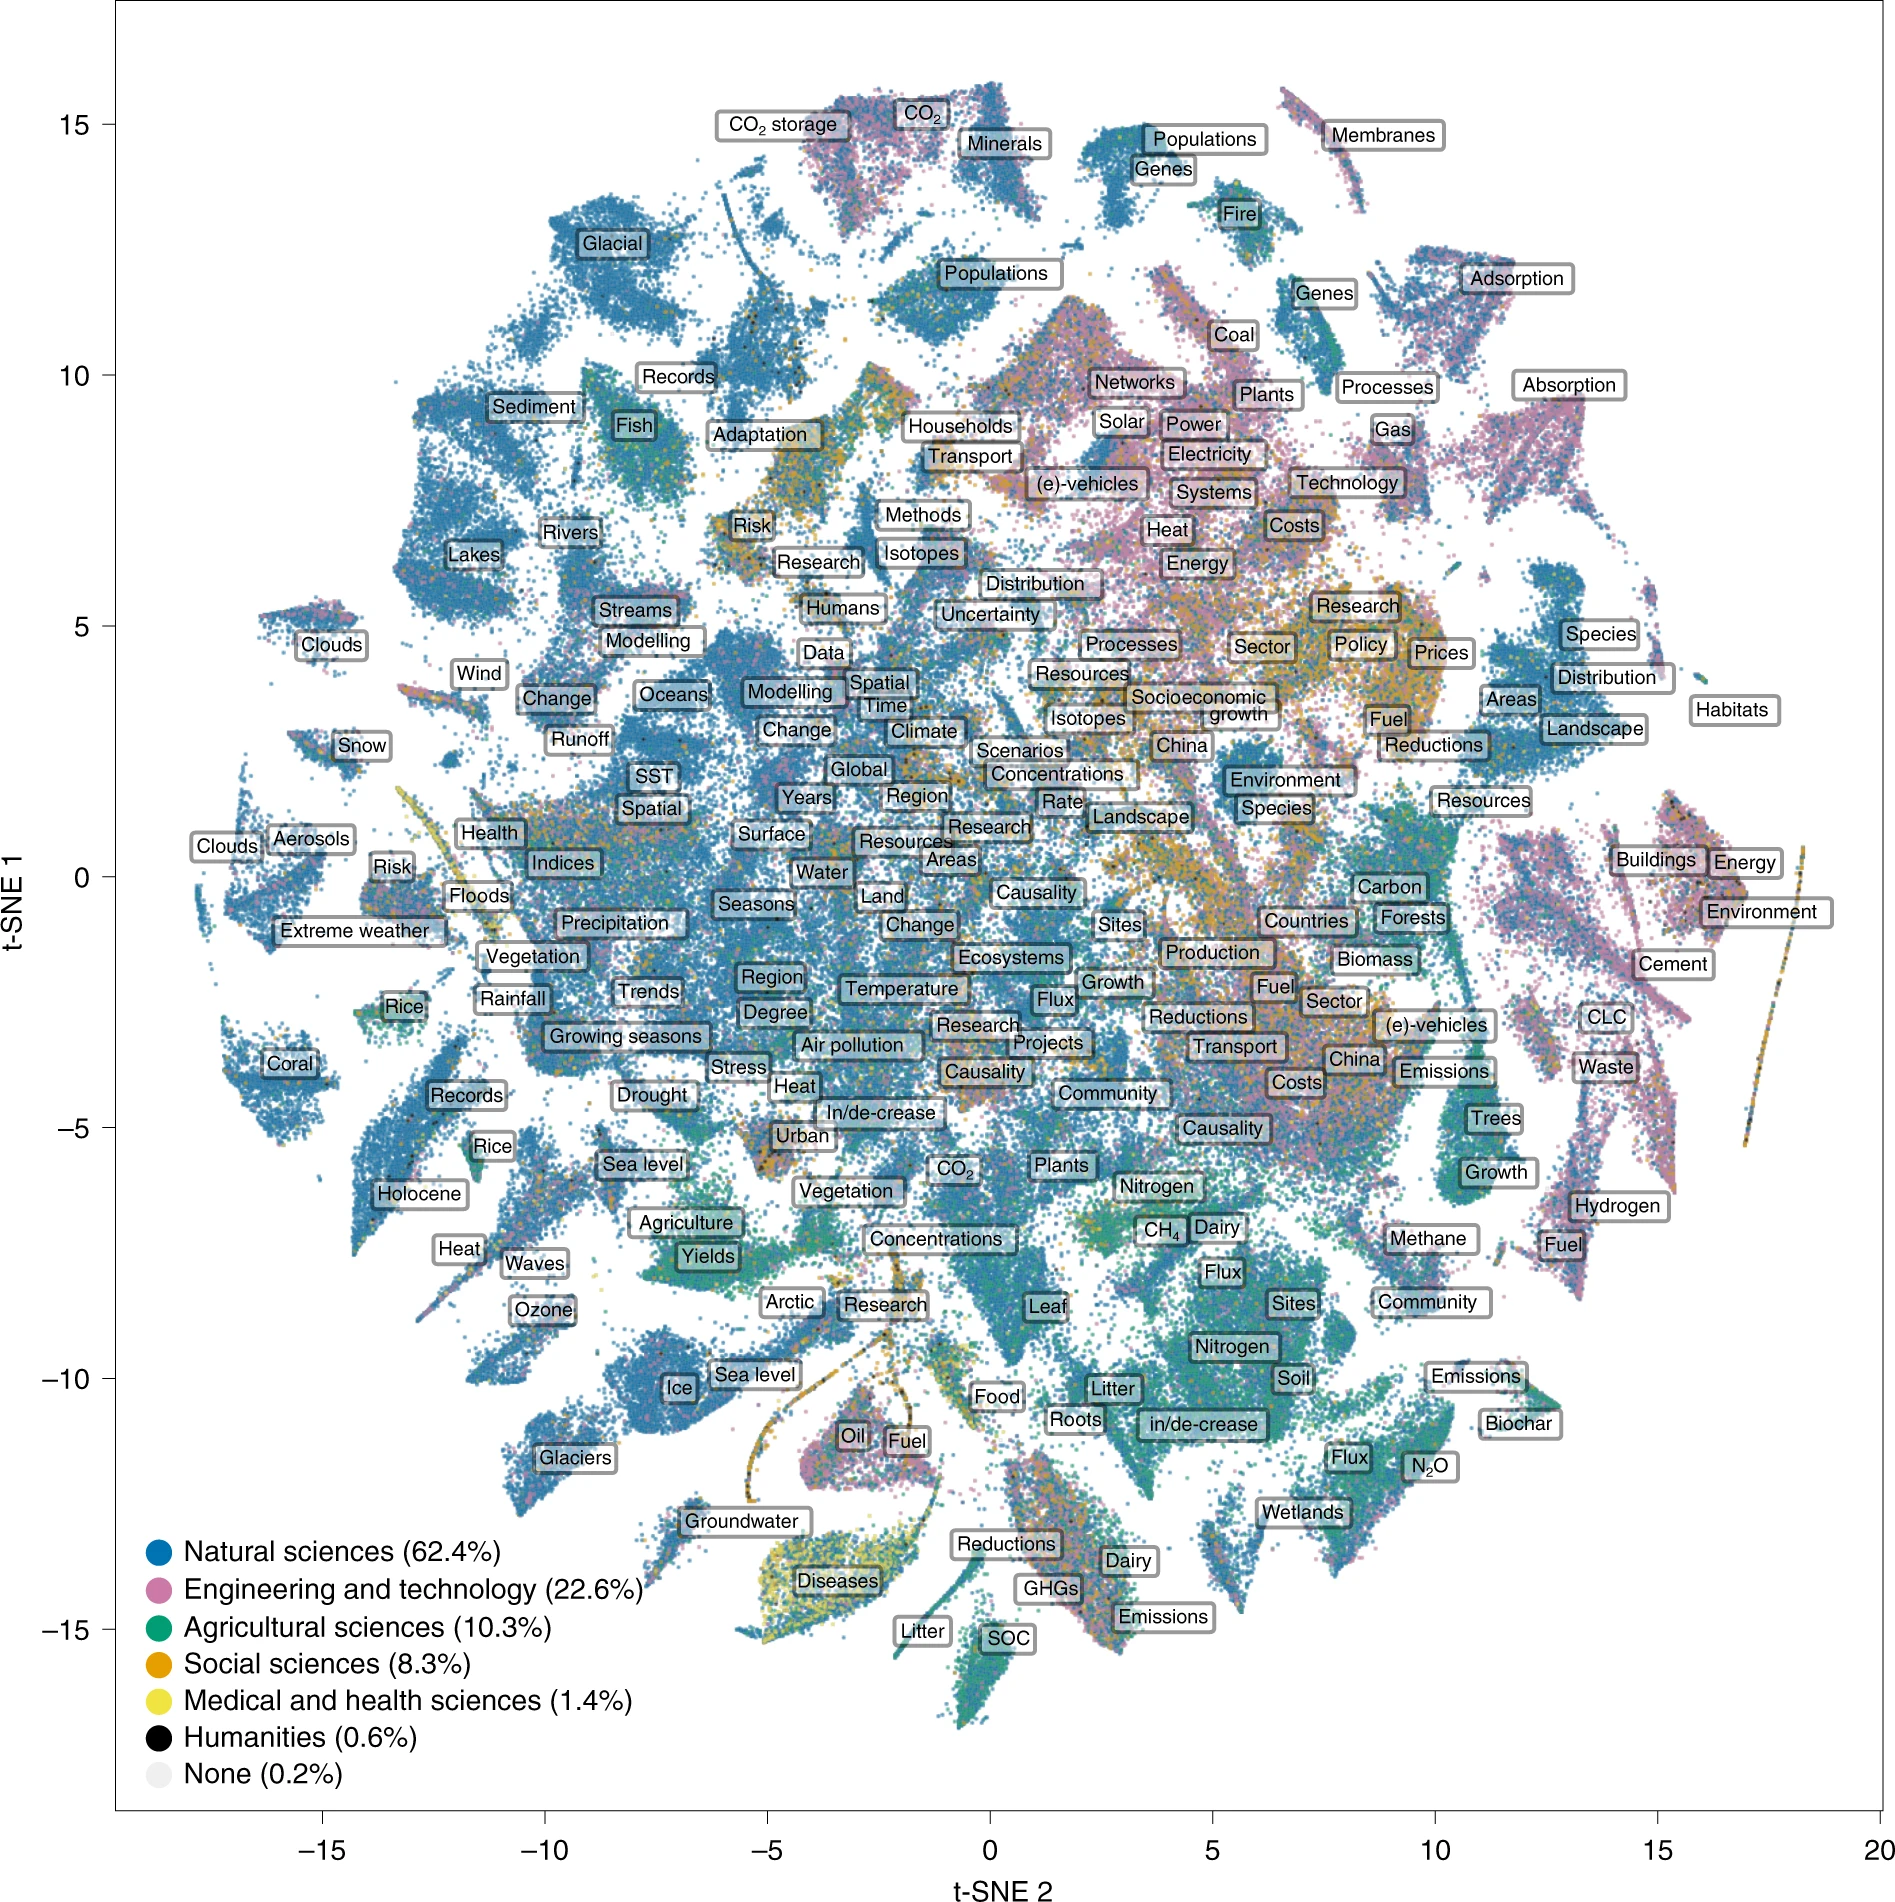
\includegraphics{images/cc_topography.png}
\end{frame}

\begin{frame}{What are plots for}
\protect\hypertarget{what-are-plots-for}{}
We do not interpret distances directly from the plot, which can quickly
resemble reading tea leaves!

In general plots show if your model space has represented something
useful in relation to other variables, and they help to explain what the
model is doing.

They are also very useful for exploring a dataset.
\end{frame}

\begin{frame}[fragile]{How can we do this}
\protect\hypertarget{how-can-we-do-this}{}
There are three common algorithms

\begin{itemize}
\tightlist
\item
  PCA
\item
  t-SNE
\item
  UMAP
\end{itemize}

UMAP represents the state-of-the-art, so let's try it out with some text
data.

\scriptsize

\begin{Shaded}
\begin{Highlighting}[]
\FunctionTok{library}\NormalTok{(readr)}
\NormalTok{df }\OtherTok{\textless{}{-}} \FunctionTok{read\_csv}\NormalTok{(}\StringTok{"data/uk\_manifestos.csv"}\NormalTok{)}
\NormalTok{corp }\OtherTok{\textless{}{-}} \FunctionTok{corpus}\NormalTok{(df)}
\NormalTok{dfmat }\OtherTok{\textless{}{-}}\NormalTok{ corp }\SpecialCharTok{\%\textgreater{}\%} \FunctionTok{tokens}\NormalTok{(}\AttributeTok{remove\_punc=}\ConstantTok{TRUE}\NormalTok{) }\SpecialCharTok{\%\textgreater{}\%}
  \FunctionTok{tokens\_remove}\NormalTok{(}\AttributeTok{pattern=}\FunctionTok{stopwords}\NormalTok{(}\StringTok{"en"}\NormalTok{)) }\SpecialCharTok{\%\textgreater{}\%}
  \FunctionTok{dfm}\NormalTok{() }\SpecialCharTok{\%\textgreater{}\%}
  \FunctionTok{dfm\_trim}\NormalTok{(}\AttributeTok{min\_termfreq=}\DecValTok{5}\NormalTok{)}
\end{Highlighting}
\end{Shaded}
\end{frame}

\begin{frame}[fragile]{Plotting UK manifestos with UMAP}
\protect\hypertarget{plotting-uk-manifestos-with-umap}{}
In R we can use the
\href{https://cran.r-project.org/web/packages/uwot/uwot.pdf}{uwot}
package, which is much faster than the
\href{https://cran.r-project.org/web/packages/umap/vignettes/umap.html}{umap}
package.

\begin{cols}

\begin{col}{0.5\textwidth}

\scriptsize

\begin{Shaded}
\begin{Highlighting}[]
\FunctionTok{library}\NormalTok{(uwot)}
\NormalTok{embeddings }\OtherTok{\textless{}{-}} \FunctionTok{umap}\NormalTok{(}\FunctionTok{as.matrix}\NormalTok{(dfmat))}
\NormalTok{df}\SpecialCharTok{$}\NormalTok{x }\OtherTok{\textless{}{-}}\NormalTok{ embeddings[,}\DecValTok{1}\NormalTok{]}
\NormalTok{df}\SpecialCharTok{$}\NormalTok{y }\OtherTok{\textless{}{-}}\NormalTok{ embeddings[,}\DecValTok{2}\NormalTok{]}

\NormalTok{colordict }\OtherTok{\textless{}{-}} \FunctionTok{c}\NormalTok{(}
  \StringTok{"Labour"}\OtherTok{=}\StringTok{"red"}\NormalTok{,}\StringTok{"LibDems"}\OtherTok{=}\StringTok{"yellow"}\NormalTok{,}
  \StringTok{"Conservatives"}\OtherTok{=}\StringTok{"Blue"}\NormalTok{,}\StringTok{"Greens"}\OtherTok{=}\StringTok{"green"}\NormalTok{)}

\NormalTok{p }\OtherTok{\textless{}{-}} \FunctionTok{ggplot}\NormalTok{(df, }\FunctionTok{aes}\NormalTok{(x, y, }\AttributeTok{fill=}\NormalTok{party)) }\SpecialCharTok{+} 
  \FunctionTok{geom\_point}\NormalTok{(}\AttributeTok{color=}\StringTok{"grey"}\NormalTok{, }\AttributeTok{shape=}\DecValTok{21}\NormalTok{, }\AttributeTok{size=}\FloatTok{0.5}\NormalTok{) }\SpecialCharTok{+} 
  \FunctionTok{scale\_fill\_manual}\NormalTok{(}\AttributeTok{values=}\NormalTok{colordict) }\SpecialCharTok{+} 
  \FunctionTok{theme\_bw}\NormalTok{() }\SpecialCharTok{+}
  \FunctionTok{coord\_fixed}\NormalTok{()}
\NormalTok{p}
\end{Highlighting}
\end{Shaded}

\begin{Shaded}
\begin{Highlighting}[]
\FunctionTok{ggsave}\NormalTok{(}\StringTok{"plots/uk\_umap.png"}\NormalTok{, }\AttributeTok{width=}\DecValTok{4}\NormalTok{, }\AttributeTok{height=}\DecValTok{4}\NormalTok{)}
\end{Highlighting}
\end{Shaded}

\end{col}

\begin{col}{0.04\textwidth}
~

\end{col}

\begin{col}{0.46\textwidth}
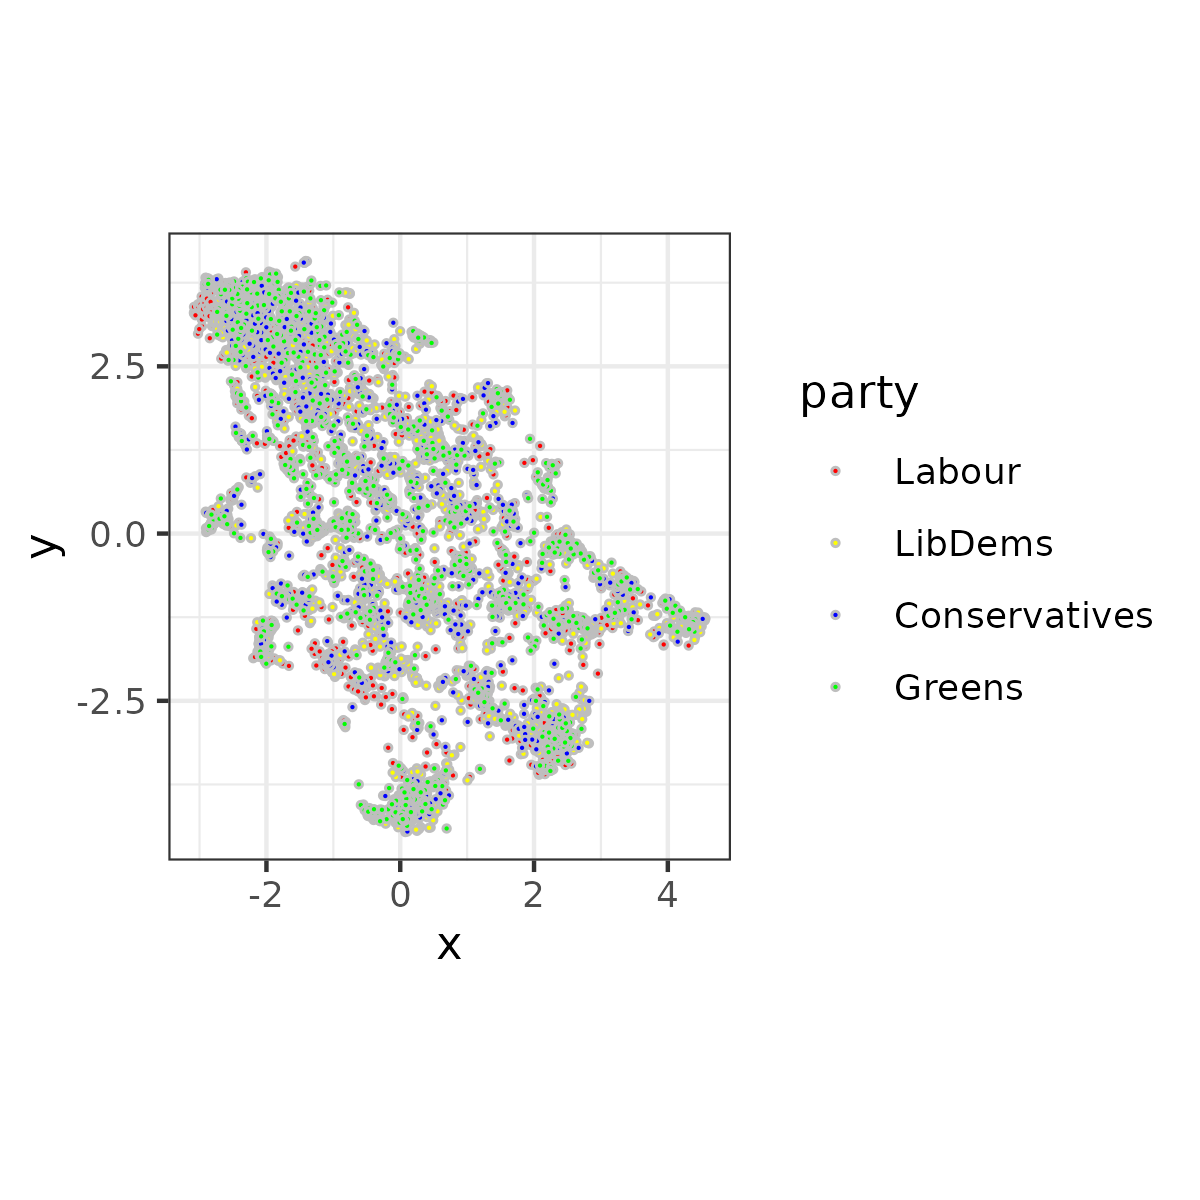
\includegraphics{plots/uk_umap.png}

\end{col}

\end{cols}
\end{frame}

\begin{frame}[fragile]{Plotting UK manifestos with UMAP in python}
\protect\hypertarget{plotting-uk-manifestos-with-umap-in-python}{}
In python we use the
\href{https://umap-learn.readthedocs.io/en/latest/}{umap-learn} package

\begin{cols}

\begin{col}{0.63\textwidth}

\scriptsize

\begin{Shaded}
\begin{Highlighting}[]
\ImportTok{import}\NormalTok{ umap}
\ImportTok{import}\NormalTok{ seaborn }\ImportTok{as}\NormalTok{ sns}
\NormalTok{df }\OperatorTok{=}\NormalTok{ pd.read\_csv(}\StringTok{"data/uk\_manifestos.csv"}\NormalTok{)}
\NormalTok{vec }\OperatorTok{=}\NormalTok{ CountVectorizer(min\_df}\OperatorTok{=}\DecValTok{5}\NormalTok{, stop\_words}\OperatorTok{=}\StringTok{"english"}\NormalTok{)}
\NormalTok{dfmat }\OperatorTok{=}\NormalTok{ vec.fit\_transform(df[}\StringTok{"text"}\NormalTok{])}
\NormalTok{cdict }\OperatorTok{=}\NormalTok{ \{}
    \StringTok{\textquotesingle{}Labour\textquotesingle{}}\NormalTok{: }\StringTok{\textquotesingle{}red\textquotesingle{}}\NormalTok{,}
    \StringTok{\textquotesingle{}LibDems\textquotesingle{}}\NormalTok{: }\StringTok{\textquotesingle{}yellow\textquotesingle{}}\NormalTok{,}
    \StringTok{\textquotesingle{}Conservatives\textquotesingle{}}\NormalTok{: }\StringTok{\textquotesingle{}blue\textquotesingle{}}\NormalTok{,}
    \StringTok{\textquotesingle{}Greens\textquotesingle{}}\NormalTok{: }\StringTok{\textquotesingle{}green\textquotesingle{}}
\NormalTok{\}}
\NormalTok{reducer }\OperatorTok{=}\NormalTok{ umap.UMAP()}
\NormalTok{embeddings }\OperatorTok{=}\NormalTok{ reducer.fit\_transform(dfmat)}
\NormalTok{df[}\StringTok{"x"}\NormalTok{] }\OperatorTok{=}\NormalTok{ embeddings[:,}\DecValTok{0}\NormalTok{]}
\NormalTok{df[}\StringTok{"y"}\NormalTok{] }\OperatorTok{=}\NormalTok{ embeddings[:,}\DecValTok{1}\NormalTok{]}
\NormalTok{sns.relplot(}
\NormalTok{  data}\OperatorTok{=}\NormalTok{df, x}\OperatorTok{=}\StringTok{"x"}\NormalTok{, y}\OperatorTok{=}\StringTok{"y"}\NormalTok{, hue}\OperatorTok{=}\StringTok{"party"}\NormalTok{, edgecolor}\OperatorTok{=}\StringTok{"grey"}\NormalTok{,}
\NormalTok{  s}\OperatorTok{=}\DecValTok{8}\NormalTok{, palette}\OperatorTok{=}\NormalTok{cdict, facet\_kws}\OperatorTok{=}\NormalTok{\{}\StringTok{"despine"}\NormalTok{: }\VariableTok{False}\NormalTok{\}}
\NormalTok{)}
\end{Highlighting}
\end{Shaded}

\begin{Shaded}
\begin{Highlighting}[]
\NormalTok{plt.savefig(}\StringTok{"plots/uk\_umap\_sns.png"}\NormalTok{)}
\end{Highlighting}
\end{Shaded}

\end{col}

\begin{col}{0.04\textwidth}
~

\end{col}

\begin{col}{0.33\textwidth}
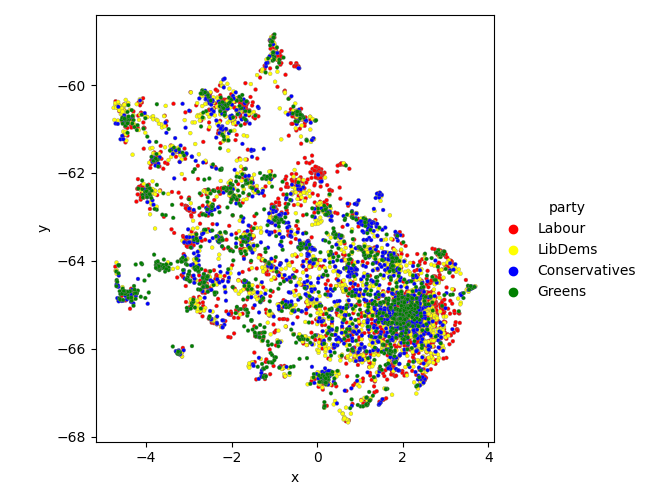
\includegraphics{plots/uk_umap_sns.png}

\end{col}

\end{cols}
\end{frame}

\begin{frame}[fragile]{Interactive plots}
\protect\hypertarget{interactive-plots}{}
We can think of this technique as allowing us to ``map'' a document
space: we \textbf{project} multidimensional data onto two dimensions.
But remember, the map is not the territory: all projections are
distortionary.

However, some projections are useful, especially if we make them
explorable by being interactive.

We can do a quick version really easily with plotly:

\scriptsize

\begin{Shaded}
\begin{Highlighting}[]
\FunctionTok{library}\NormalTok{(plotly)}
\NormalTok{p }\OtherTok{\textless{}{-}} \FunctionTok{ggplot}\NormalTok{(df, }\FunctionTok{aes}\NormalTok{(x, y, }\AttributeTok{colour=}\NormalTok{party, }\AttributeTok{label=}\NormalTok{text)) }\SpecialCharTok{+} 
  \FunctionTok{geom\_point}\NormalTok{(}\AttributeTok{size=}\FloatTok{0.5}\NormalTok{) }\SpecialCharTok{+} 
  \FunctionTok{scale\_colour\_manual}\NormalTok{(}\AttributeTok{values=}\NormalTok{colordict) }\SpecialCharTok{+} 
  \FunctionTok{theme\_bw}\NormalTok{() }\SpecialCharTok{+}
  \FunctionTok{coord\_fixed}\NormalTok{()}

\FunctionTok{ggplotly}\NormalTok{(p)}
\end{Highlighting}
\end{Shaded}
\end{frame}

\begin{frame}[fragile]{Interactive plots in python}
\protect\hypertarget{interactive-plots-in-python}{}
We can make some nice interactive plots in python with
\href{https://docs.bokeh.org/en/latest/index.html}{Bokeh}:

\tiny

\begin{Shaded}
\begin{Highlighting}[]
\ImportTok{from}\NormalTok{ bokeh.plotting }\ImportTok{import}\NormalTok{ figure, show, output\_notebook}
\ImportTok{from}\NormalTok{ bokeh.models }\ImportTok{import}\NormalTok{ HoverTool, ColumnDataSource, CategoricalColorMapper}
\ImportTok{from}\NormalTok{ bokeh.palettes }\ImportTok{import}\NormalTok{ Spectral10}

\NormalTok{output\_notebook()}

\NormalTok{datasource }\OperatorTok{=}\NormalTok{ ColumnDataSource(df)}
\NormalTok{color\_mapping }\OperatorTok{=}\NormalTok{ CategoricalColorMapper(}
\NormalTok{    palette}\OperatorTok{=}\BuiltInTok{list}\NormalTok{(cdict.values()),}
\NormalTok{    factors}\OperatorTok{=}\BuiltInTok{list}\NormalTok{(cdict.keys())}
\NormalTok{)}

\NormalTok{plot\_figure }\OperatorTok{=}\NormalTok{ figure(}
\NormalTok{    title}\OperatorTok{=}\StringTok{\textquotesingle{}UMAP projection of UK manifestos\textquotesingle{}}\NormalTok{,}
\NormalTok{    plot\_width}\OperatorTok{=}\DecValTok{600}\NormalTok{,plot\_height}\OperatorTok{=}\DecValTok{600}\NormalTok{,}
\NormalTok{    tools}\OperatorTok{=}\NormalTok{(}\StringTok{\textquotesingle{}pan, wheel\_zoom, reset\textquotesingle{}}\NormalTok{)}
\NormalTok{)}

\NormalTok{plot\_figure.add\_tools(HoverTool(}
\NormalTok{    tooltips}\OperatorTok{=}\StringTok{"\textless{}span\textgreater{}@text\textless{}/span\textgreater{}"}
\NormalTok{))}

\NormalTok{plot\_figure.circle(}
    \StringTok{\textquotesingle{}x\textquotesingle{}}\NormalTok{,}\StringTok{\textquotesingle{}y\textquotesingle{}}\NormalTok{,source}\OperatorTok{=}\NormalTok{datasource,}
\NormalTok{    fill\_color}\OperatorTok{=}\BuiltInTok{dict}\NormalTok{(field}\OperatorTok{=}\StringTok{\textquotesingle{}party\textquotesingle{}}\NormalTok{, transform}\OperatorTok{=}\NormalTok{color\_mapping),}
\NormalTok{    line\_color}\OperatorTok{=}\StringTok{"grey"}\NormalTok{,line\_alpha}\OperatorTok{=}\FloatTok{0.6}\NormalTok{,fill\_alpha}\OperatorTok{=}\FloatTok{0.6}\NormalTok{,size}\OperatorTok{=}\DecValTok{4}
\NormalTok{)}
\NormalTok{show(plot\_figure)}
\end{Highlighting}
\end{Shaded}
\end{frame}

\begin{frame}{Exercise}
\protect\hypertarget{exercise-1}{}
Take your document you selected earlier. Find the similar documents in
the 2-dimensional space. Are these still close together? What are the
similarity scores in the 2 dimensional space?
\end{frame}

\hypertarget{wrapup-and-outlook}{%
\section{Wrapup and outlook}\label{wrapup-and-outlook}}

\begin{frame}{Wrapup}
\protect\hypertarget{wrapup}{}
We have delved deeper into multidimensional feature representations of
documents.

In this multidimensional space, we can now say how similar a pair of
documents are. For examples of this in action, have a look at
\href{https://static1.squarespace.com/static/5dc421b1359959419cd251d4/t/60186ce591c77159e8caa357/1612213506614/Farrell_NCC_Climate2016.pdf}{this
paper} by Justin Farrell, which tries to use similarity to understand
the similarity of congress, presidential speeches, and news texts about
climate change to contrarian actors.
\end{frame}

\begin{frame}{Outlook}
\protect\hypertarget{outlook}{}
Next week we'll look at word and document embeddings.

Here we represent words themselves as multidimensional vectors.

Embeddings extend our ``bag of words'' model, and form the basis of much
of modern NLP
\end{frame}

\begin{frame}[allowframebreaks]{}
  \bibliographytrue
  \bibliography{../presentation-resources/MyLibrary.bib}
\end{frame}

\end{document}
